%% AMS-LaTeX Created with the Wolfram Language : www.wolfram.com

\documentclass{article}
\usepackage{amsmath, amssymb, graphics, setspace}

\newcommand{\mathsym}[1]{{}}
\newcommand{\unicode}[1]{{}}

\newcounter{mathematicasection}
\newcounter{mathematicasubsection}
\newcounter{mathematicasubsubsection}
\begin{document}

\title{Durable goods and installed base degradation via software updates}
\author{Abstract}
\date{}
\maketitle

In this paper we study a monopolist technology vendor{'}s decision to degrade their installed base when they release their newer version. An installed
base of products that are technologically tethered, whether digital products such as smartphones or predominantly non-digital products such as automobiles,
can be degraded in performance through software updates. This raises new possibilities and temptations for sellers, and therefore new questions not
hitherto addressed in the literature on durable goods and innovation, on the optimal product policy for durable goods monopolists. In contrast to
the traditional planned obsolescence literature, where the seller has to introduce novel versions (novel in either fashion or functional features)
to obsolete the older versions, in the changed scenario when a seller can degrade their installed base via a software update, they don{'}t have to
rely on product novelty to encourage consumers to buy the new product. In a two-period setting featuring a monopolist selling a durable good to a
unit mass of consumers with uniformly distributed valuation for the good, we show evidence that installed base degradation can emerge in equilibrium,
with or without innovation. In the absence of innovation (i.e. same durable good available for sale in both periods), our model first finds that
the seller is mostly better off not degrading their older version in period 2, except for products with very low marginal cost relative to value,
which should be leased and not sold. Nevertheless, the seller faces a commitment problem and is tempted to degrade the new version in period 2, for
a substantial part of the parameter space. { }Next, in the presence of innovation, we find that the seller is better off not degrading the earlier
version in the later period, when the marginal cost is high relative to product value, and innovation is low, or when marginal cost is very low and
innovation is very high. But there exists a substantial region in the middle, when marginal cost is low, and innovation is high, when the seller
earns a higher profit overall by degrading their period-1 version in period 2, { }which explains why durable goods vendors may face incentives to
engage in this practice. With innovation as well, there exists a region in the parameter space where the seller faces a commitment problem and achieves
sub-optimal profit by degrading their period-1 product in period 2, when they could earn a higher profit by refraining from doing so. In the no-innovation
scenario, installed base degradation is mostly sub-optimal to the seller due to the commitment problem, whereas in the innovation scenario, installed
base degradation is mostly optimal with a relatively smaller sub-optimal region.

\section*{Introduction}

In 2018 (? - check), Apple was accused of deliberately slowing down the existing older versions of iPhones, when they introduced the newer iPhone
15 (? - check). After much controversy, Apple confirmed this: according to Forbes magazine, {``}Following significant examination and documentation
by third parties, Apple has confirmed that its software does degrade the performance of older iPhones. This is, according to the statement, undertaken
in {`}a bid to deliver the best experience for its customers{'}. That may be the case, but it is a trick that Apple has not been open about.{''}
(https://www.forbes.com/sites/ewanspence/2017/12/20/apple-iphone-kill-switch-ios-degrade-cripple-performance-battery/$\#$f6cf61216a85) 

In this paper, we show that a durable goods monopolist does face a significant incentive to degrade or disable the performance of their previous
version, when they introduce their subsequent version. More surprisingly, we show that under some conditions, this can happen even if it is sub-optimal
for the seller{'}s profit: even if the seller is better off not degrading the product, they may do so. The link between the above action by Apple
and our paper is: Companies such as Apple may be facing a temptation to degrade its older version when its newer version hits the market, even though
that was not Apple{'}s intention earlier.\\
\\
In the industry examples discussed above, degradation is not complete - a customer can still (barely) use their older iPhone, even though it is significantly
slower. However, for practical purposes, the slow response of the iPhone wears on the customer, and they eventually yield and buy the new iPhone.
Our analysis captures this notion, and models the degradation of the installed base as a complete degradation - i.e. in period 2, when the seller
degrades the installed base, its utility decreases to zero.

\section*{Literature}

Companies like Apple have incentives to degrade prior-period versions during subsequent periods, to increase profits. We show that profits do increase.
We also show that there exist some conditions when the profit is actually lower with degrading than without, but the seller faces a commitment problem
and is unable to refrain from degrading their earlier version. Durable goods vendors face a time-inconsistency problem (Coase, 1972), because durable
goods sold in future periods affect the value of goods sold in prior periods. This limits the seller{'}s profits (Stokey, 1981). We see evidence
of this time-inconsistency problem: in our results, the period-1 optimal action for period-2 is different from the period-2 optimal action.\\
\\
Selling for a durable goods vendor has been shown to induce competition with existing installed base, which drives down price (Coase, 1972). We incorporate
this feature in our model: in period-2, consumers compare their value from upgrading to their value from continuing to use the older version, where
available. Therefore, the seller faces a potential incentive to degrade the older version, in order to minimize the competition with the later version.
\\
\\
Anticipation of lower prices causes consumers to hold off on purchases, putting further price pressure (Bhaskaran and Gilbert, 2005; Coase, 1972).
We incorporate this feature in our model: the first-period buyers weigh their benefit from buying in period 1, versus waiting and buying from period
2. Finally, leasing has been identified as an alternative for the vendor to improve their profits (Bhaskaran and Gilbert, 2005). We derive conditions
under which leasing is a viable alternative.\\
\\
Ex-ante planned obsolescence, wherein firms produce {``}durable{''} goods with uneconomically short lives, which break down earlier than they should
(Bulow, 1986) - so as to induce customers to make repeat purchases - have been well studied in the literature. Planned obsolescence could also be
induced ex post (Waldman, 1993), in subsequent periods - when vendors can introduce newer versions whose very presence can obsolete the older versions
due to fashion (e.g. newer model cars putting older models out of fashion) or technological incompatibility (newer version of a software causing
older versions to become unable to open files produced by the newer version), and so on. \\
\\
Our work is consistent with (Waldman, 1993) in looking at the seller{'}s incentive to depreciate the prior version when introducing the new version.
However, there is a major difference. Our work asks what would happen if the seller is able to degrade or disable the older version by a software
update, when the newer version is introduced. From an economic and marketing viewpoint, this new phenomenon is different from the planned obsolescence
as identified by (Waldman, 1993): if the seller can degrade performance with software based updates, then product obsolescence is delinked from the
incremental value delivered by the newer product. This leads us to map the optimality of product obsolescence by varying the incremental value. \\
\\
Incremental value can be decomposed into two dimensions: one is the incremental value of the new version compared to the older version, and the other
is the incremental value of the older version relative to the marginal cost. We leverage both these dimensions for enhanced insight, and explore
the optimality of the decision to degrade, in a parameter space with varying levels of incremental innovation (high versus low) and varying levels
of { }intrinsic product value relative to marginal cost (again, high versus low). Surprisingly, we find that under some conditions, this obsoleting
of the prior version actually hurts the seller{'}s profit - they are better off not engaging in this action, but may lack the ability to commit to
the optimal decision.\\
\\
The phenomenon of selling damaged durable goods has been studied before (Deneckere and McAfee, 1996; Hahn, 2006). Hahn (2006) studies damaged goods
- i.e. the main product offered as a crimped version, offered simultaneously with the main version, or sequentially after the main version - can
help alleviate the Coasian time inconsistency problem. Another way to eliminate the competition between different versions of durable goods, is to
damage or disable the previous version when the new version is introduced. Our work explores this aspect by studying durable goods that are rendered
completely unusable (rather than partially damaged) in future periods, when new versions are introduced. 

\section*{Discussion of assumptions}

From equation 19, when seller innovates but does not degrade: 

\begin{doublespace}
\noindent\(\pmb{\theta _{12}>\theta _1>\theta _2\forall \left\{\frac{3}{2} v_1>v_2>v_1>\frac{9}{8}c>0\right\}}\)
\end{doublespace}

\(\text{Case} (B-\text{ii}): \left(0<\theta _2<\theta _1<1\right)\text{When} \text{seller} \text{degrades}\)

\begin{doublespace}
\noindent\(\pmb{\theta _2<\theta _1\forall \left\{v_2>v_1>\frac{9}{8}c>0\right\}}\)
\end{doublespace}

When the seller introduces an upgrade \(v_2\), they are assumed to charge the same price \(p_2\) to all buyers of \(v_2\). All products have a marginal
cost \(c\) that does not change with version. The rationale is that the materials involved in the manufacture are essentially the same.

\section*{Outline of analysis}

We first analyze the case where the monopolist does not innovate (section 5). We find that mostly, as at the start of the two-period time horizon,
the seller is better off not degrading product quality (section 5.3), but in period 2, the seller is tempted to degrade the product quality (section
5.4). \\
\\
Next, we analyze the case where the monopolist does innovate (section 6). Here, { }we first compute the seller{'}s profit expression when they degrade
their initial version in period 2 (section 6.1). \\
\\
Then we compute their profit when they don{'}t degrade (section 6.2). In this case, we find that the seller sells to the same set of consumers in
both periods, but is unable to commit to their optimal-profit sales strategy.\\
\\
When marginal cost is low relative to value and innovation is high, { }as at the start of the time horizon under consideration, degrading the period-1
product in period-2 is the optimal strategy for the seller. This explains why companies like Apple may be tempted to degrade the performance of their
earlier iPhone versions when they release newer versions.\\
\\
Interestingly, for a significant subset of the parameter space, the seller faces a commitment problem in period 2 and ends up degrading their older
version when they should optimally not do so. In other words, the seller sub-optimally faces temptation to degrade their older version when they
release their newer version, even though they can earn higher profit overall by not doing so. Technology vendors should be aware of this potential
drawback. \\
\\
On the other hand, when marginal cost is high and innovation is low, the seller does not face this problem, and is better off leasing the product,
which is consistent with the prior findings conventional durable goods literature. 

\section*{When monopolist does not innovate}

Here we consider the base case when the product involves no innovation, but is sold over two periods. We show that when the durable good is not subject
to innovation, and when \(v>>c\) (specifically, \(v>10c\)) it is better for monopolist to degrade the product after each period, rather than not
(i.e. \(\left.\pi _n<\pi _d\right)\). However, at the start of each period, the seller is subject to a different set of incentives: { }(i) at the
start of period 1, when \(10c>v>c\), the monopolist is better off not degrading the product in period 2 (i.e. \(\pi _n>\pi _d\)); nevertheless (ii)
in period 2, when \(v>\frac{5}{4}c\), the monopolist faces incentives in period 2, to crimp their product so as to encourage more sales (i.e. \(\pi
_{\text{d2}}>\pi _{\text{n2}}\)). Combining the two analyses, we find that in fig.$\_\_\_$, in region (I), when \(v>10c\), we have \(\pi _n<\pi _d\)
and \(\pi _{\text{n2}}<\pi _{\text{d2}}\), so that it is always optimal for the seller to degrade. In region (II), when \(10c>v>\frac{5}{4}c\), we
have \(\pi _n>\pi _d\) and \(\pi _{\text{n2}}<\pi _{\text{d2}}\), so that it is optimal for the seller to not degrade their first-period product
in period 2, but at the start of period 2 the seller nevertheless faces an incentive to degrade their initial version, forcing consumers to purchase
the same product again. Rational forward looking consumers expect this behavior, and it decreases their willingness to pay in period 1. In region
(III), when \(\frac{5}{4}c>v>c\), { }we have \(\pi _n>\pi _d\) and \(\pi _{\text{n2}}>\pi _{\text{d2}}\), so that it is optimal for the seller to
not degrade their product, either in period 1 or period 2. In the no-innovation situation, it is never the case that (\(\pi _n<\pi _d\) and \(\pi
_{\text{n2}}>\pi _{\text{d2}}\)) - i.e. that the seller is overall better off degrading their product, but faces an incentive to not degrade in period
2. (As we will see later, this last condition does not hold for the case of innovation.)

Our analysis in this section proceeds as follows. Section 5.1 (case A) derives the seller{'}s overall profit and period-2 profit when they sell \(v\)
in period 1, and does not degrade it in period 2 (i.e. the period 1 product can be used for two periods). Section 5.2 (case B) computes the seller{'}s
overall profit and period-2 profit when they sell v in period 1, but degrade it in period 2, so that it can only be used for one period. We compare
the overall profits and period-2 profits under the above conditions, to derive regions (see fig.0 $\_\_\_$) where (I) \(\pi _n<\pi _d\) and \(\pi
_{\text{n2}}<\pi _{\text{d2}}\), (II) \(\pi _n>\pi _d\) and \(\pi _{\text{n2}}<\pi _{\text{d2}}\), and (III) \(\pi _n>\pi _d\) and \(\pi _{\text{n2}}>\pi
_{\text{d2}}\), and discuss findings and implications.

\subsection*{Case (A): Monopolist does not degrade period-1 bought v in period 2}

Since the product purchased in period 1 continues to be useful in period 2, period-1 buyers will continue to use it in period 2. Since there is no
innovation, consumers \(\left[\theta _1,1\right]\) who bought in period 1 will not buy in period 2. Some \(\left.\left[\theta _2,\theta _1\right.\right)\)
customers who bought nothing in period 1 will buy v in period 2. \\
\\
In period 2, the threshold customer \(\theta _2\) is indifferent between (buying v at price \(p_2\)) and (buying nothing), which is given by the
indifference equation \(\theta _2v-p_2=0\). We set the seller{'}s optimal \(p_2=v \theta _2\) in the seller{'}s second period profit \(\pi _2=\left(p_2-c\right)\left(\theta
_1-\theta _2\right)\), and solve the first order condition \(\frac{\partial \pi _2}{\partial \theta _2}=0\) to obtain the optimal \(\theta _2^*=\frac{c+v
\theta _1}{2 v}\).

In period 1, the threshold customer \(\theta _1\) is indifferent between (i) buying v at price \(p_1\) and using it for two periods, and (ii) waiting,
and buying v at price \(p_2\) in period 2. This implies the following indifference equation: \(\theta _1 (2 v) - p_1 = \theta _1 v - p_2\), which
yields the optimal \(p_1=\frac{1}{2} \left(c+3 v \theta _1\right)\). We substitute for this \(p_1\) in the seller{'}s optimal period-1 profit \(\pi
_1=\left(p_1-c\right)\left(1-\theta _1\right)\). 

The overall profit (subscript {``}n{''} to denote that case that the seller is not degrading the older version) is given by the sum of the profit
over each period: \(\pi _n=\pi _1+\pi _2\). Solving the first order condition \(\frac{\partial \pi _n}{\partial \theta _1}=0\) for the optimal \(\theta
_1\) that maximizes overall profit over both periods, we obtain \(\theta _1=\frac{3}{5}\), and \(\theta _2=\frac{3}{10}+\frac{c}{2 v}\). We now substitute
the optimal \(\theta _1\) and \(\theta _2\) values into the profit expression to compute the total optimal profit, over both periods:

\begin{equation}
\pi _n=\frac{1}{20} \left(-10 c+\frac{5 c^2}{v}+9 v\right)
\end{equation}

We then use the optimal $\theta $ values to compute the second-period profit expression:

\begin{equation}
\pi _{\text{n2}}=\frac{(5 c-3 v)^2}{100 v}
\end{equation}

Both of the above profit expressions are subscripted by {``}n{''} to refer to the case where the seller does not degrade the older version in the
second period.

\subsection*{Case (B): Monopolist does degrade v}

This time, we consider the case when the monopolist does degrade v in period 2.

As before, we proceed with period 2 analysis first. Since the seller depreciates \(v\) in period 2, customers who bought \(v\) in period 1 will buy
\(v\) again in period 2. In each period, there is only one cutoff customer: \(\theta _1\) in period 1, and \(\theta _2\) in period 2. We show that,
since \(v_2=v_1\), it follows that \(\theta _2=\theta _1\) as well. The threshold customer \(\theta _2\) is indifferent between (i) buying v at price
\(p_2\) and (ii) buying nothing, which yields the following indifference equation: \(\theta _2v-p_2=0\). Solving for \(p_2\) yields { }\(p_2=v \theta
_2\), which we substitute in the seller{'}s second period profit: \(\pi _2=\left(p_2-c\right)\left(1-\theta _2\right)\). Solving the first order
condition \(\frac{\partial \pi _2}{\partial \theta _2}=0\) yields the optimal \(\theta _2=\frac{c+v}{2 v}\), which yields the second period profit
\(\pi _{\text{d2}}\) (we now append the subscript {``}d{''} to denote that this is the case where the seller degrades the initial version in period
2):

\begin{equation}
\pi _{\text{d2}}=\frac{(v-c)^2}{4 v}
\end{equation}

The first period is no different from the second period, in that the product v sold in period 1 at price \(p_1\) will be used only for one period.
The buyer will (by construction) degrade it in period 2, and consumers will expect it to be degraded. Hence, \(p_1=p_2\), and hence \(\theta _1=\theta
_2\). Therefore, the seller chooses \(p_1=\frac{c+v}{2}\), and optimizes their first period profit \(\pi _1=\left(p_1-c\right)\left(1-\theta _1\right)\).
Solving the first order condition \(\frac{\partial \pi _1}{\partial \theta _1}=0\) for optimal \(\theta _1\), we get \(\theta _1=\frac{c+v}{2 v}\).
Substituting \(p_1\), \(\theta _1\) into the expression for \(\pi _{\text{d1}}\), we get 

\begin{equation}
\pi _{\text{d1}}=\frac{(v-c)^2}{4 v}
\end{equation}

The overall profit therefore is 

\begin{equation}
\pi _d =\pi _{\text{d1}}+\pi _{\text{d2}}=\frac{(v-c)^2}{2 v}
\end{equation}

\subsection*{Comparison of overall profit for the two cases}

Comparing equations (1) and { }(5) for \(\pi _n\) and \(\pi _d\) respectively (shown below), from the point of view of maximizing overall profit:
\(\pi _n>\pi _d\) when \(10 c>v>c\) (region (II) in figure $\_\_\_$), suggesting that with no innovation, at the start of period 1, there exists
a range of intermediate parameter values where it is optimal for the seller to refrain from degrading their first-period product in period 2. In
other words, when the marginal cost c is somewhat large compared to product utility v (to the highest type customer), the seller is { }better off
not degrading when the product is subject to no innovation. (Example: iPhones. Costs about $\$$280, retails for about $\$$700). \\
\\
However there exists a small region (I) (figure $\_\_\_$) with very low marginal cost relative to product value (\(v>10 c\)) , where it is better
for overall profit for the seller to degrade the period-1 version in period 2. This corresponds to the classic leasing result in durable goods literature.
In the case of software, this suggests the use of subscription.\\
\\
Region (III) (figure $\_\_\_$) is infeasible because the value of the product to the customer with the highest valuation \((\theta =1)\) is lower
than the marginal cost: \(v<c\).

\[\pi _n=\frac{1}{20} \left(-10 c+\frac{5 c^2}{v}+9 v\right)\\
\\
\pi _d =\frac{(v-c)^2}{2 v}\]

\begin{equation}
\pi _n>\pi _d \forall \{9 c> v>c>0\}
\end{equation}

\begin{equation}
\pi _n<\pi _d \forall \{v>10c>0\}
\end{equation}

\begin{doublespace}
\noindent\(\pmb{\text{RegionPlot}\left[\left\{\pi _n>\pi _d ,v>c\right\},\{c,0.0001,20\},\{v,0.0001,20\},\text{FrameLabel}\to \{\text{c},\text{v}\},\right.}\\
\pmb{\text{Epilog}\to \{}\\
\pmb{\text{Text}[\text{Style}[\text{I},18],\text{Scaled}[\{0.05,0.9\}]],}\\
\pmb{\text{Text}[\text{Style}[\text{{``}II{''}},15],\text{Scaled}[\{0.3,0.6\}]],}\\
\pmb{\text{Text}[\text{Style}[\text{{``}III{''}},15],\text{Scaled}[\{0.8,0.6\}]]\}}\\
\pmb{]}\)
\end{doublespace}

\includegraphics{2020_05_19-overleaf-mirror_gr1.eps}

\subsection*{Per.2 Profit comparison (A) vs (B)}

Comparing equations (2) and (3), it can be shown in region (I) of figure $\_\_\_$, that when \(v>\frac{5}{4}c\), we have \(\pi _{\text{n2}}<\pi _{\text{d2}}\),
suggesting that with no innovation, at the start of period 2, the seller faces a temptation to degrade the version 1 in period 2: their profit from
degrading in period 2 \(\left(\pi _{\text{d2}}\right.\)) exceeds their profit from not degrading in period 2 \(\left(\pi _{\text{n2}}\right.\)).
\\
\\
In region (II) of figure $\_\_\_$, when \(c<v<\frac{5}{4}c\), we have \(\pi _{\text{n2}}>\pi _{\text{d2}}\) : at lower levels of value relative to
marginal cost, it does not make sense for the seller to degrade the installed base in period 2. 

\[\pi _{\text{n2}}=\frac{(5 c-3 v)^2}{100 v}\\
\\
\pi _{\text{d2}}=\left(-c+\frac{c+v}{2}\right) \left(1-\frac{c+v}{2 v}\right)\]

\begin{equation}
\pi _{\text{n2}}<\pi _{\text{d2}} \forall \left\{v > \frac{5}{4}c > 0\right\}
\end{equation}

\begin{equation}
\pi _{\text{n2}}>\pi _{\text{d2}} \forall \left\{\frac{5}{4}c>v > c > 0\right\}
\end{equation}

\begin{doublespace}
\noindent\(\pmb{\text{RegionPlot}\left[\left\{\pi _{\text{n2}}<\pi _{\text{d2}} ,v >\text{  }c\right\},\{c,0.0001,20\},\{v,0.0001,20\},\text{FrameLabel}\to
\{\text{c},\text{v}\},\text{Epilog}\to \{\right.}\\
\pmb{\text{Text}[\text{Style}[\text{I},18],\text{Scaled}[\{0.3,0.7\}]],}\\
\pmb{\text{Text}[\text{Style}[\text{{``}II{''}},15],\text{Scaled}[\{0.63,0.7\}]]\}]}\)
\end{doublespace}

\includegraphics{2020_05_19-overleaf-mirror_gr2.eps}

\subsection*{Superimposing optimal actions of both periods}

Superimposing the two graphs, we find that when the product utility v (to the highest type customer) vis-a-vis the marginal cost is in the range
\(\frac{5}{4}c<v<10c\), the seller faces a commitment problem: at the start of period 2, the seller is { }better off degrading the installed base
in period 2, whereas at the start of period 1, the seller is better off preserving the installed base in period 2. In the range \(v>10c\), the seller
faces uniform incentives - in period 1 and period 2 - to degrade the installed base in period 2. In both of the above cases, the observed outcome
is that the seller degrades the installed base in period 2, which is consistent with observed practice in industry.\\
\\
However, when \(c<v<\frac{5}{4}c\), the seller again faces uniform incentives - in period 1 and period 2 - to preserve the installed base in period
2, while continuing to sell to newer customers in period 2. For this smaller region, when v is not much larger than c, in the second period it is
not optimal to depreciate the older version, because the gain from additional sales (each sale yielding only a small margin) does not compensate
for the lost sales from previous period consumers who defer purchasing, anticipating future depreciation. (REWORD)\\
\\
This analysis therefore throws light on why sellers might sometimes act to degrade their installed base, and at other times act to preserve their
installed base.

\begin{doublespace}
\noindent\(\pmb{\text{RegionPlot}\left[\left\{\pi _n>\pi _d,\pi _{\text{n2}}<\pi _{\text{d2}} ,v >\text{  }c\right\},\{c,0.0001,20\},\{v,0.0001,20\},\text{FrameLabel}\to
\{\text{c},\text{v}\},\right.}\\
\pmb{\text{Epilog}\to \{\text{Text}[\text{Style}[\text{I},18],\text{Scaled}[\{0.05,0.8\}]],\text{Text}[\text{Style}[\text{{``}II{''}},15],\text{Scaled}[\{0.3,0.8\}]],}\\
\pmb{\text{Text}[\text{Style}[\text{{``}III{''}},15],\text{Scaled}[\{0.7,0.8\}]],}\\
\pmb{\text{Text}[\text{Style}[\text{{``}IV{''}},15],\text{Scaled}[\{0.9,0.8\}]]}\\
\pmb{\}]}\)
\end{doublespace}

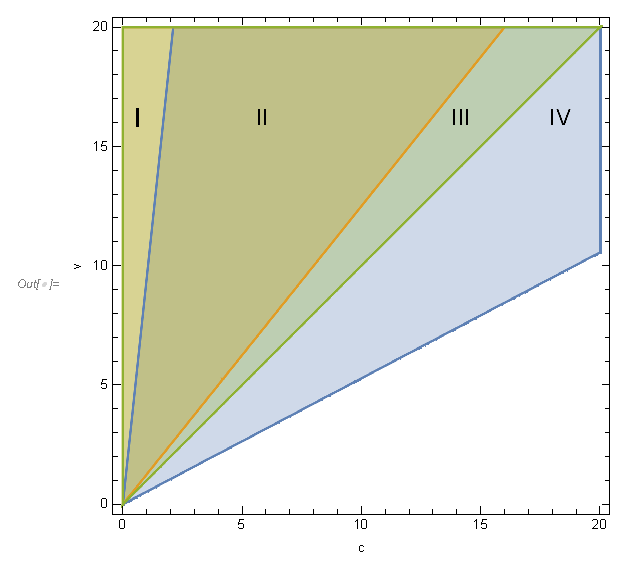
\includegraphics{2020_05_19-overleaf-mirror_gr3.eps}

\pmb{ Theorem:} \\
For the case of no-innovation:\\
Region I: Seller is better off degrading the product in period 2, as at the start of period 1 as well as period 2 { }- the classic durable goods
result. Degrading the product is optimal in both first and second periods. This points to the leasing or subscription outcome which is profit maximizing
for the firm.\\
Region II: Seller is better off not degrading their product in period 2, as at the start of period 1, but at the start of period 2 they face a temptation
to degrade their product. Consumers expect this outcome and lower their willingness to pay for the initial version, and this hurts the seller{'}s
profit.\\
Region III: Seller is better off not degrading their product in period 2 (same as region II), as at the start of period 1, and they are not tempted
to degrade it in period 2 either (unlike region II). This suggests the {``}sale{''} outcome, or a longer leasing horizon or subscription window.
\\
Region IV: Here the value of the product is less than its marginal cost, so the product is not sold. 

\section*{When monopolist innovates }

Seller incurs a marginal cost \(c\) per unit sold, same as the no-innovation case. 

\subsection*{Case (A): When seller does not degrade \(v_1\) in period 2}

In this scenario, in period 2, all period 1 purchases are worth their previous value. Nevertheless, some { }period 1 buyers \(\left.\left[\theta
_{12},1\right.\right)\) may be in the market to upgrade to the new version whose value is \(v_2\). Another set of buyers \(\left.\left[\theta _2,\theta
_1\right.\right)\) buy the new version \(v_2\) in period 2, without having bought anything in period 1. We assume that \(\theta _{12}>\theta _1>\theta
_2\) and derive the following results. Then we verify that the assumption \(\theta _{12}>\theta _1>\theta _2\) is satisfied, for the parameter region
of interest. The seller chooses \(\theta _{12}\) and \(\theta _2\) to optimize their second period profit, which we derive as follows.

 In period 2, the cutoff \(\theta _2\) buyer is indifferent between (i) buying \(v_2\) at price \(p_2\), and (ii) buying nothing, which yields the
indifference equation: 

\begin{equation}
v_2 \theta _2-p_2 = 0
\end{equation}

We substitute for \(p_2=v_2\theta _2\) in the cutoff \(\theta _{12}\) buyer{'}s indifference equation. This buyer is indifferent between (i) buying
\(v_2\) at price \(p_2\), and (ii) buying nothing and continuing to use \(v_1\) in period 2, which yields the indifference equation \(\theta _{12}v_2-p_2=\theta
_{12}v_1\), which can be re-written as:

\begin{equation}
\theta _{12}v_2-v_2\theta _2=\theta _{12}v_1
\end{equation}

Solving the above equation, we get \(\theta _{12}=\frac{v_2 \theta _2}{v_2-v_1}\). Substituting for \(\theta _{12}\) in the equation for the seller{'}s
second period profit \(\pi _{\text{n2}}=\left(p_2-c\right)\left(\theta _1-\theta _2\right)+\left(p_2-c\right)\left(1-\theta _{12}\right)\), and solving
the first order condition \(\frac{\partial \pi _2}{\partial \theta _2}=0\), we obtain the optimal values for \(\theta _2\) and \(\theta _{12}\):


\begin{equation}
\theta _2=\frac{-c v_1+2 c v_2-v_1 v_2+v_2^2-v_1 v_2 \theta _1+v_2^2 \theta _1}{2 v_2 \left(-v_1+2 v_2\right)}
\end{equation}

\begin{equation}
\theta _{12}=\frac{-c v_1+2 c v_2-v_1 v_2+v_2^2-v_1 v_2 \theta _1+v_2^2 \theta _1}{2 \left(v_1-2 v_2\right) \left(v_1-v_2\right)}
\end{equation}

Substituting \(\theta _2\) and \(\theta _{12}\) in the seller{'}s second period profit expression yields the following simplified expression:

\begin{equation}
\pi _{\text{n2}}=\frac{\left(v_1 \left(c-v_2 \left(1+\theta _1\right)\right)+v_2 \left(-2 c+v_2 \left(1+\theta _1\right)\right)\right){}^2}{4 \left(v_1-2
v_2\right) \left(v_1-v_2\right) v_2}
\end{equation}

In period 1, the threshold customer \(\theta _1\) is { }indifferent between (i) buying \(v_1\) at price \(p_1\) and using it for two periods, and
(ii) waiting and buying \(v_2\) in period 2. The indifference equation is given by: \(2 \theta _1v_1 - p_1 = \theta _1 v_2 - p_2\) . Substituting
\(p_2=v_2\theta _2\) where \(\theta _2\) is given by equation 12 and simplifying, we obtain:

\begin{equation}
p_1=\frac{c v_1-2 c v_2+v_1 v_2-v_2^2+4 v_1^2 \theta _1-9 v_1 v_2 \theta _1+3 v_2^2 \theta _1}{2 \left(v_1-2 v_2\right)}
\end{equation}

The seller{'}s period-1 profit expression is given by \(\pi _{\text{n1}}=\left(p_1-c\right)\left(1-\theta _1\right)\) . We add this to \(\pi _{\text{n2}}\)
given by equation 14 and solve the first order condition \(\frac{\partial \left(\pi _1+\pi _2\right)}{\partial \theta _1}=0\) to obtain the optimal
\(\theta _1\):

\begin{equation}
\theta _1=\frac{4 v_1^2-9 v_1 v_2+3 v_2^2}{8 v_1^2-19 v_1 v_2+7 v_2^2}
\end{equation}

Substituting for this \(\theta _1\) in equation 14, the second period profit is therefore given by:

\begin{equation}
\pi _{\text{n2}}=\frac{\left(4 v_1^3 \left(2 c-3 v_2\right)+v_1 \left(45 c-38 v_2\right) v_2^2+2 v_2^3 \left(-7 c+5 v_2\right)+5 v_1^2 v_2 \left(-7
c+8 v_2\right)\right){}^2}{4 \left(v_1-2 v_2\right) \left(v_1-v_2\right) v_2 \left(8 v_1^2-19 v_1 v_2+7 v_2^2\right){}^2}
\end{equation}

Total profit simplifies to:

\begin{equation}
\pi _n=\frac{1}{196} \left(7 \left(\frac{7 c^2}{v_2}+6 v_2+7 c \left(-4+\frac{c}{-v_1+v_2}\right)\right)+v_1 \left(51+v_1 \left(\frac{49}{v_1-2 v_2}-\frac{4
\left(4 v_1+v_2\right)}{8 v_1^2-19 v_1 v_2+7 v_2^2}\right)\right)\right)
\end{equation}

We algebraically verify that for the region of interest, \(\theta _{12}>\theta _1>\theta _2\):

\begin{equation}
\theta _{12}>\theta _1>\theta _2\forall \left\{\frac{3}{2} v_1>v_2>v_1>\frac{9}{8}c>0\right\}
\end{equation}

\subsection*{Case (B): When seller degrades \(v_1\) in period 2}

The seller has several choices: They can (i) sell less to period-2 consumers than period-1 consumers: \(\theta _2>\theta _1\), or (ii) sell more
to period-2 consumers than period-1 consumers: \(\theta _2<\theta _1\), or (iii) sell the same period-2 optimal quantity to period-1 consumers: \(\theta
_1=\theta _2=\theta _2^*\), or (iv) sell an optimal quantity denoted by a cutoff customer \(\theta _0^*\): \(\theta _1=\theta _2=\theta _0^*\).\\
\hspace*{0.5ex} \\
Regarding (i), as we show in appendix, \(\theta _2>\theta _1\) does not emerge in equilibrium: having chosen a \(\theta _1\) in period 1, the \(\theta
_2\) - optimal cutoff customer in period 2 - is independent of period 1 { }cutoff \(\theta _1\). Therefore, having chosen a \(\theta _1\) in period
1, the seller chooses \(\theta _2<\theta _1\) (alternative (ii) dominates (i)). \\
\\
We show that the seller can make a higher profit with (iii) - in period 1, if they choose \(\theta _1=\theta _2^*\), they make a higher profit overall
than if they choose \(\theta _1=\theta _1^*\), so that (ii) is dominated by (iii). \\
\\
Finally, we show that there exists a cutoff customer \(\theta _0^*>\theta _2^*\), which results in even higher overall profit - but the seller is
unable to commit to selling at \(\theta _0^*\): having chosen \(\theta _0\) in period 1, the seller deviates and offers \(\theta _2\) in period 2
(because second period profit from deviating is higher: \(\pi _{2\theta _2}>\pi _{2\theta _0}\)), even though sticking to a \(\theta _0\) schedule
in both periods would have been optimal overall \(\left(\pi _{\theta _0}>\pi _{\theta _2}\right)\). Anticipating this, the consumers and seller converge
on (ii): the \(\theta _2<\theta _1\) strategy, which is dominated by (iii): \(\theta _1=\theta _2=\theta _2^*\).\\
\\
Therefore, only (c) \(\theta _1=\theta _2=\theta _2^*\) is the equilibrium outcome.

\subsubsection*{\(0<\theta _1<\theta _2<1\) is infeasible }

Lemma: Selling to more consumers in period 1 and fewer consumers in period 2 - i.e. \(\left(\theta _1,1\right)\) { }in period 1 and { }\(\left(\theta
_2,1\right)\) in period 2, where \(0<\theta _1<\theta _2<1\), is not a feasible outcome. { } 

\pmb{ Proof:} 

In period 2, all period 1 purchases are worthless. That means, all period 1 buyers will be in the market to buy again.

In period 2, the cutoff \(\theta _2\) buyer is indifferent between (i) buying \(v_2\) at price \(p_2\), and (ii) buying nothing, which yields the
indifference equation: \(v_2 \theta _2-p_2 = 0\) . We solve for \(p_2\), substitute it in the seller{'}s period-2 profit expression: \(\pi _2=\left(p_2-c\right)\left(1-\theta
_2\right)\) , and solve the first order condition \(\frac{\partial \pi _2}{\partial \theta _2}=0\) to obtain the optimum \(\theta _2=\frac{c+v_2}{2
v_2}\).

In period 1, the cutoff \(\theta _1\) buyer is indifferent between (i) buying \(v_1\) at price \(p_1\), and (ii) buying nothing, since \(0<\theta
_1<\theta _2<1\) by assumption. This { }yields the indifference equation: \(\theta _1v_1 - p_1 =0\) . We obtain \(p_1=\theta _1v_1\), substitute
it in the seller{'}s period-1 profit expression: \(\pi _1=\left(p_1-c\right)\left(1-\theta _1\right)\) , and solve the first order condition \(\frac{\partial
\pi _1}{\partial \theta _1}=0\) to obtain the optimum \(\theta _1=\frac{c+v_1}{2 v_1}\). 

\(\text{Since} v_2>v_1 , \text{it} \text{follows} \text{that}\text{  }\frac{c+v_1}{2 v_1}>\frac{c+v_2}{2 v_2}.\) Hence, \(\theta _1>\theta _2\),
which contradicts our starting assumption that \(0<\theta _1<\theta _2<1\).

\subsubsection*{\(0<\theta _2<\theta _1<1\) is feasible}

In this scenario, in period 2, all period 1 purchases are worthless. All period 1 buyers will be in the market in period 2 to buy again.

In period 2, the cutoff \(\theta _2\) buyer is indifferent between (i) buying \(v_2\) at price \(p_2\), and (ii) buying nothing, which yields the
indifference equation: \(v_2 \theta _2-p_2 = 0\) . We solve for \(p_2\), substitute it in the seller{'}s period-2 profit expression: \(\pi _2=\left(p_2-c\right)\left(1-\theta
_2\right)\) , and solve the first order condition \(\frac{\partial \pi _2}{\partial \theta _2}=0\) to obtain the optimum \(\theta _2=\frac{c+v_2}{2
v_2}\). The seller profit in period 2 simplifies to: \(\pi _{\text{d2}\left(\theta _1,\theta _2\right)}=\frac{\left(c-v_2\right){}^2}{4 v_2}\).

In period 1, the cutoff \(\theta _1\) buyer is indifferent between (i) buying \(v_1\) at price \(p_1\), and (ii) waiting and buying \(v_2\) in period
2, because \(\theta _2<\theta _1\) by assumption. This { }yields the indifference equation: \(\theta _1v_1 - p_1 = \theta _1 v_2 - p_2\) . We obtain
\(p_1=\frac{1}{2} \left(c+v_2+2 v_1 \theta _1-2 v_2 \theta _1\right)\), substitute it in the seller{'}s period-1 profit expression: \(\pi _1=\left(p_1-c\right)\left(1-\theta
_1\right)\) , and solve the first order condition \(\frac{\partial \pi _1}{\partial \theta _1}=0\) to obtain the optimum \(\theta _1=-\frac{-c-2
v_1+3 v_2}{4 \left(v_1-v_2\right)}\). The seller profit in period 2 simplifies to: \(\pi _{\text{d1}\left(\theta _1,\theta _2\right)}=\frac{\left(c-2
v_1+v_2\right){}^2}{16 \left(v_1-v_2\right)}\).

We verify that the derived expressions for \(\theta _1=-\frac{-c-2 v_1+3 v_2}{4 \left(v_1-v_2\right)}\) and \(\theta _2=\frac{c+v_2}{2 v_2}\) satisfy
our assumption that \(\theta _2<\theta _1\forall \left\{v_2>v_1>\frac{9}{8}c>0\right\}\).

Over both periods, the seller{'}s total profit simplifies to: 

\begin{equation}
\pi _{d\left(\theta _1,\theta _2\right)}=\pi _{\text{d1}}+\pi _{\text{d2}}=\frac{-4 c v_1 \left(c-3 v_2\right)-4 v_1^2 v_2+\left(c-3 v_2\right) \left(3
c-v_2\right) v_2}{16 v_2 \left(-v_1+v_2\right)}
\end{equation}

\subsubsection*{\(0<\theta _1=\theta _2=\theta _2^*<1\) dominates \(0<\theta _2<\theta _1<1\) }

Here we set \(\theta _1=\theta _2=\theta _2^*\), and show that the seller earns a higher profit that the earlier case of \(0<\theta _2<\theta _1<1\).

In period 2, the cutoff \(\theta _2\) buyer is indifferent between (i) buying \(v_2\) at price \(p_2\), and (ii) buying nothing, which yields the
indifference equation: \(v_2 \theta _2-p_2 = 0\) . We solve for \(p_2\), substitute it in the seller{'}s period-2 profit expression: \(\pi _2=\left(p_2-c\right)\left(1-\theta
_2\right)\) , and solve the first order condition \(\frac{\partial \pi _2}{\partial \theta _2}=0\) to obtain the optimum \(\theta _2^*=\frac{c+v_2}{2
v_2}\). The seller profit in period 2 simplifies to: \(\pi _{\text{d2}\left(\theta _2,\theta _2\right)}=\frac{\left(c-v_2\right){}^2}{4 v_2}\).

\begin{equation}
\pi _{\text{d2}\left(\theta _2,\theta _2\right)}=\frac{\left(c-v_2\right){}^2}{4 v_2}
\end{equation}

In period 1, the cutoff \(\theta _1\) buyer is indifferent between (i) buying \(v_1\) at price \(p_1\), and (ii) buying nothing, because \(\theta
_1=\theta _2\) by assumption. This { }yields the indifference equation: \(\theta _2v_1 - p_1 = 0\) . We obtain \(p_1=\theta _2v_1=\frac{c+v_2}{2
v_2}v_1\), substitute it in the seller{'}s period-1 profit expression: \(\pi _{\text{d1}}=\left(p_1-c\right)\left(1-\theta _2\right)\) , which simplifies
to:

\begin{equation}
\pi _{\text{d1}\left(\theta _2,\theta _2\right)}=\frac{\left(c-v_2\right) \left(2 c v_2-v_1 \left(c+v_2\right)\right)}{4 v_2^2}
\end{equation}

Over both periods, the total profit simplifies to:

\begin{equation}
\pi _{d\left(\theta _2,\theta _2\right)}=\pi _{\text{d1}\left(\theta _2,\theta _2\right)}+\pi _{\text{d2}\left(\theta _2,\theta _2\right)}=\frac{\left(v_2-c\right)
\left(v_2 \left(-3 c+v_2\right)+v_1 \left(c+v_2\right)\right)}{4 v_2^2}
\end{equation}

Lemma: The seller is better off selling to the same set of consumers \(\left(\theta _2,1\right)\) in both periods, than to a different set of consumers
\(\left(\theta _1,1\right)\) in period 1, followed by \(\left(\theta _2,1\right)\) in period 2. 

\pmb{ Proof:} 

Comparing the seller{'}s profit from (a) selling to the same set of consumers \(\left(\theta _2,1\right)\) in both periods (equation 23) to (b) than
from selling to a different set of consumers \(\left(\theta _1,1\right)\) in period 1, followed by \(\left(\theta _2,1\right)\) in period 2 (equation
20), we verify that \(\pi _{d\left(\theta _2,\theta _2\right)}>\pi _{d\left(\theta _1,\theta _2\right)}\)simplifies to \(\left(2 c v_1+v_2 \left(-3
c+v_2\right)\right){}^2>0\) which is always true for all \(v_2>v_1>c>0\).

\subsubsection*{\(0<\theta _1=\theta _2=\theta _0^*<1\) dominates \(0<\theta _1=\theta _2=\theta _2^*<1\) but seller cannot commit}

We now explore whether the seller could improve their overall profit by choosing some \(\theta _0\neq \theta _2\) as the common cutoff consumer for
both periods. Therefore we set \(\theta _1=\theta _2=\theta _0^*\).

In period 2, the cutoff \(\theta _2=\theta _0\) buyer is indifferent between (i) buying \(v_2\) at price \(p_2\), and (ii) buying nothing, which
yields the indifference equation: \(v_2 \theta _0-p_2 = 0\) . We solve for \(p_2\), and substitute it in the seller{'}s period-2 profit expression:
\(\pi _{\text{d2}}=\left(p_2-c\right)\left(1-\theta _0\right)\) . Unlike the earlier analysis, this time we don{'}t solve the first order condition
\(\frac{\partial \pi _{\text{d2}}}{\partial \theta _0}=0\), but rather solve the overall profit function over both periods: \(\frac{\partial \left(\pi
_{\text{d1}}+\pi _{\text{d2}}\right)}{\partial \theta _0}=0\) to obtain the optimum \(\theta _0\). For this, we need to compute the first period
profit \(\pi _{\text{d1}}\) as well, as shown next.

In period 1, the cutoff \(\theta _1\) buyer is indifferent between (i) buying \(v_1\) at price \(p_1\), and (ii) buying nothing, because \(\theta
_1=\theta _0\) by assumption. This { }yields the indifference equation: \(\theta _0v_1 - p_1 = 0\) . We obtain \(p_1=\theta _0v_1\), and substitute
it in the seller{'}s period-1 profit expression: \(\pi _{\text{d1}}=\left(p_1-c\right)\left(1-\theta _0\right)\).

Over both periods, the total profit expression is given by { }\(\pi _{d\left(\theta _0,\theta _0\right)}=\left(1-\theta _0\right) \left(-2 c+\left(v_1+v_2\right)
\theta _0\right)\), whose first order condition \(\frac{\partial \pi _d}{\partial \theta _0}=0\) when solved for \(\theta _0\) yields \(\theta _0=\frac{2
c+v_1+v_2}{2 \left(v_1+v_2\right)}\). Substituting, we obtain the following expression for the total profit:

\begin{equation}
\pi _{\text{d1}\left(\theta _0,\theta _0\right)}=\frac{\left(-2 c+v_1+v_2\right) \left(v_1^2+\left(-2 c+v_1\right) v_2\right)}{4 \left(v_1+v_2\right){}^2}
\end{equation}

\begin{equation}
\pi _{\text{d2}\left(\theta _0,\theta _0\right)}=\frac{1}{4} \left(v_2+2 c \left(-1+\frac{2 c v_1}{\left(v_1+v_2\right){}^2}\right)\right)
\end{equation}

\begin{equation}
\pi _{d\left(\theta _0,\theta _0\right)}=\pi _{\text{d1}}+\pi _{\text{d2}}=\frac{\left(-2 c+v_1+v_2\right){}^2}{4 \left(v_1+v_2\right)}
\end{equation}

\pmb{ Proposition: }When the seller innovates but degrades their older product, in period 1, the seller chooses a fixed \(\theta _1=\theta _2=\theta
_2^*\) in equilibrium, even though they could earn a higher profit by choosing a fixed \(\theta _1=\theta _2=\theta _0^*\).

The seller earns a higher profit by setting cutoff customers of both periods \(\theta _1\) and \(\theta _2\) to the higher identical value \(\theta
_0^*=\frac{2 c+v_1+v_2}{2 \left(v_1+v_2\right)}\), compared to the lower identical value \(\theta _2^*=\frac{c+v_2}{2 v_2}\)

\pmb{ Proof: }First, we show that \(\theta _2^*<\theta _0^*\): \(\frac{c+v_2}{2 v_2}<\frac{2 c+v_1+v_2}{2 \left(v_1+v_2\right)}\) simplifies to \(c
v_2 \left(v_1+v_2\right)>0\) which is always true for all \(v_2>v_1>c>0\). Next, we show that \(\pi _{d\left(\theta _0,\theta _0\right)}>\pi _{d\left(\theta
_2,\theta _2\right)}\):\(\frac{\left(-2 c+v_1+v_2\right){}^2}{4 \left(v_1+v_2\right)}>\frac{\left(v_2-c\right) \left(v_2 \left(-3 c+v_2\right)+v_1
\left(c+v_2\right)\right)}{4 v_2^2}\) simplifies to \(c^2 v_2^2 \left(v_1+v_2\right)>0\) which again is always true for all \(v_2>v_1>c>0\).

In period 2, the seller nevertheless earns a higher profit with \(\theta _2=\theta _2^*\), and hence chooses this option, rather than \(\theta _2=\theta
_0^*\), which highlights the commitment problem faced by the seller - they are unable to stick to their optimal profit choice \(\theta _2=\theta
_0^*\) in period 2. 

\pmb{ Proof:} We show that \(\pi _{\text{d2}\left(\theta _2,\theta _2\right)}>\pi _{\text{d2}\left(\theta _0,\theta _0\right)}\): \(\frac{\left(c-v_2\right){}^2}{4
v_2}>\frac{1}{4} \left(v_2+2 c \left(-1+\frac{2 c v_1}{\left(v_1+v_2\right){}^2}\right)\right)\) simplifies to \(c^2 v_2 \left(v_1+v_2\right){}^2>0\)
which is always true for all \(v_2>v_1>c>0\). 

\subsection*{Comparison - no degrade with degrade case with innovation}

Is the seller better of degrading?

We now compare the total profit from the no-degrade case (equation 18) to the degrade-case (equation 23). We expect higher profit for the no-degrade
case (equation 18).

\[\pi _n=\frac{1}{196} \left(7 \left(\frac{7 c^2}{v_2}+6 v_2+7 c \left(-4+\frac{c}{-v_1+v_2}\right)\right)+v_1 \left(51+v_1 \left(\frac{49}{v_1-2
v_2}-\frac{4 \left(4 v_1+v_2\right)}{8 v_1^2-19 v_1 v_2+7 v_2^2}\right)\right)\right)\]

\[\pi _{d\left(\theta _2,\theta _2\right)}=\frac{\left(v_2-c\right) \left(v_2 \left(-3 c+v_2\right)+v_1 \left(c+v_2\right)\right)}{4 v_2^2}\]

For analytical simplicity we transform the variables as below:

\begin{equation}
\eta  =\frac{v_2}{v_1}
\end{equation}

Where $\eta $ is a measure of the extent of innovation (the extent to which \(v_2>v_1\)), and

\begin{equation}
\gamma =\frac{v_1}{c}
\end{equation}

Where $\gamma $ is a measure of the marginal revenue (the extent to which product value is greater than marginal cost).

We get the following simplified expressions:

\begin{equation}
\pi _d=\frac{(-1+\gamma  \eta ) (1+\eta  (-3+\gamma +\gamma  \eta ))}{4 \gamma  \eta ^2}c
\end{equation}

\begin{equation}
\pi _n=\frac{1}{4}\text{  }\left(-4+\frac{\frac{1}{-1+\eta }+\frac{1}{\eta }}{\gamma }+\frac{4 \gamma  \left(-4+3 (-2+\eta ) \eta  \left(-2+\eta
^2\right)\right)}{(-1+2 \eta ) (8+\eta  (-19+7 \eta ))}\right)c
\end{equation}

\subsection*{Results}

We now plot regions where \(\pi _n>\pi _d\) (after cancelling c on both expressions) along the dimensions of the extent of innovation (\(\eta  =\frac{v_2}{v_1}\))
on y-axis against the marginal revenue per sale (\(\gamma =\frac{v_1}{c}\)) on the x-axis (please see fig. $\_\_\_$ below). In regions where the
extent of innovation is low and marginal revenue is low (shaded), we find that \(\pi _n>\pi _d\): the optimal decision for the seller, at the start
of both periods, is to avoid degrading \(v_1\) in period 2. For the rest of the region, it is optimal for the seller to choose to degrade \(v_1\)
in period 2. This is consistent with the literature on durable goods leasing, which finds that optimally, a seller of durable goods should lease
their product in order to maximize revenues, and avoid competing with their earlier versions in later periods.

\includegraphics{2020_05_19-overleaf-mirror_gr4.eps}

Next we consider which way the seller{'}s incentives lean at the start of the second period. For this, we need to compare the seller{'}s second period
profits from degrading (\(\pi _{\text{d2}}\) from equation 21) vs not degrading (\(\pi _{\text{n2}}\) from equation 17). As before, we substitute
\(\eta  =\frac{v_2}{v_1}\) and \(\gamma =\frac{v_1}{c}\)for tractability.

\[\pi _{\text{d2}}=\frac{ (-1+\gamma  \eta )^2}{4 \gamma  \eta }c\]

\[\pi _{\text{n2}}=\frac{(8+\eta  (-35+(45-14 \eta ) \eta +2 \gamma  (-1+\eta ) (6+\eta  (-14+5 \eta ))))^2}{4 \gamma  (-1+\eta ) \eta  (-1+2 \eta
) (8+\eta  (-19+7 \eta ))^2}c\]

We now plot the region where \(\pi _{\text{d2}}>\pi _{\text{n2}}\) along the dimensions of the extent of innovation (\(\eta =\frac{v_2}{v_1}\)) on
y-axis against the marginal revenue per sale (\(\gamma =\frac{v_1}{c}\)) on x-axis (please see fig. $\_\_\_$ below). In regions where the extent
of innovation is high and marginal revenue is high (shaded), we find that \(\pi _{\text{d2}}>\pi _{\text{n2}}\): the optimal decision for the seller,
at the start of period 2, is to degrade \(v_1\) in period 2. For the rest of the region - for very low as well as very high levels of marginal revenue
and innovation, it is not optimal for the seller to choose to degrade \(v_1\) in period 2. This too is consistent with the literature on durable
goods leasing, which finds that optimally, a seller of durable goods should lease their product in order to maximize revenues, and avoid competing
with their earlier versions in later periods.

\includegraphics{2020_05_19-overleaf-mirror_gr5.eps}

\begin{doublespace}
\noindent\(\pmb{\text{RegionPlot}\left[\left\{\pi _n>\pi _d\right\},\{\gamma ,1,10\},\{\eta ,1,2\},\text{FrameLabel}\to \left\{\text{$\texttt{"}\gamma
$=}\frac{v_1}{c}\texttt{"},\text{$\texttt{"}\eta $=}\frac{v_2}{v_1}\texttt{"}\right\},\right.}\\
\pmb{\text{Epilog}\to \{\text{Text}[\text{Style}[\text{{``}Both periods{''}},18],\text{Scaled}[\{0.5,0.9\}]],\text{Text}[\text{Style}[\text{{``}Degrade{''}},15],\text{Scaled}[\{0.5,0.5\}]],}\\
\pmb{\text{Text}[\text{Style}[\text{{``}Preserve{''}},15],\text{Scaled}[\{0.20,0.1\}]]\}]}\)
\end{doublespace}

Next we combine the two results to obtain the following graph.

\includegraphics{2020_05_19-overleaf-mirror_gr6.eps}

In the above graph, \\
\\
1. Region 1 is when {``}Preserve{''} is the seller{'}s optimal decision at the start of period 1 (from fig.$\_\_\_$), as well as at the start of
period 2 (from fig.$\_\_\_$). This is observed for products with (a) high marginal cost relative to value, which therefore lowers the marginal profit
per unit sold: this makes intuitive sense, because when marginal cost is high relative to product value, that leaves little value for the buyer to
switch from a previous to a newer version; and (b) low incremental value relative to initial value - i.e. low extent of innovation - which therefore
is insufficient to draw previous-period buyers to upgrade to the newer version. \\
\\
2. Region 2 is when {``}Degrade is the optimal decision at the start of period 2, but Preserve is the optimal decision at the start of period 1.
This suggests the presence of a commitment problem - the seller acts to Degrade in period 2, when their overall profit could have been maximized
by choosing Preserve.\\
\\
Here, the observed outcome is that the seller degrades the previous version, though that is shown to be sub-optimal to the profit from not degrading
the prior version. That is, the seller is unable to commit to the profit-maximizing choice and ends up hurting their profit, by degrading the previous
version in the later period.\\
\\
3. Region 3 is when {``}Degrade{''} is the seller{'}s optimal decision at the start of period 1, as well as at the start of period 2. This is observed
for products with (a) low marginal cost relative to value, which therefore increases the marginal profit per unit sold, and intensifies the seller{'}s
incentive to force prior-period buyers to upgrade (and therefore induces the {``}degrade{''} decision), and (b) high incremental value relative to
initial value - i.e. high extent of innovation - which gives previous-period buyers more reason to upgrade to the newer version.\\
\\
This result demonstrates that sellers do have a strong incentive to degrade their earlier versions when they introduce newer versions, which is not
inconsistent with Apple{'}s alleged crimping of earlier versions of iPhones.\\
\\
4. Region 4 is when {``}Degrade{''} is optimal at the start of period 1, but {``}Preserve{''} is optimal in period 2. This suggests that the seller
is better off committing to {``}Degrade{''} option in period 1, by contractually offering a lease rather than sale. \\
\\
Interestingly, this highlights the existence of a region where the seller is explicitly required to offer a lease, and therefore also highlights
the region (3 above) where the seller, though not required to offer a lease, adopts a product release policy that is de facto equivalent to a lease.
Why might a seller not announce a lease? Because that leaves the possibility for greater profit than that obtained in region 3, due to the presence
of myopic consumers who go ahead and purchase???

\section*{Conclusions and discussion }

\subsection*{Summary of findings}

In summary, we find that there are conditions under which a monopolist seller of durable goods can find it optimal to degrade their installed base
in a subsequent period, both in the presence and absence of innovation. In the absence of innovation, when the intrinsic value of the product exceeds
a certain cutoff marginal cost, degrading the installed base is the equilibrium outcome. Furthermore, for a substantial part of this region, when
the intrinsic value is below an upper threshold of marginal cost, degrading the installed base is sub-optimal for the seller. When the intrinsic
value is above a higher marginal cost cutoff, degrading the installed base is optimal for the seller. In the absence of innovation, when the intrinsic
value of the product is below a certain cutoff marginal cost, it is optimal for the seller to preserve the value of the installed base.\\
\\
In the presence of innovation, when the intrinsic value is high with respect to marginal cost (i.e. relative marginal cost is low), and when the
intrinsic value of the upgrade is high with respect to the intrinsic value of the initial version (i.e. innovation is high), it is optimal for the
seller to degrade the installed base. For high relative marginal cost and low innovation levels, the seller is better off preserving the installed
base in period 2. For intermediate levels of relative marginal cost and innovation levels, the seller faces a commitment problem: their equilibrium
outcome is to degrade their installed base, but their profit maximizing outcome is to preserve their installed base. For low relative marginal cost
and high innovation levels, the seller is better off degrading the installed base in period 2. However, this is not a stable equilibrium, because
in period 2, the seller faces incentives to continue with the older version. To avoid this, the seller should commit to leasing the product, rather
than selling it.

\subsection*{Managerial implications and further research}

Durable goods vendors can use the framework of figure $\_\_\_$ to estimate where they are in terms of their relative marginal cost versus innovation
levels. For example, from news articles, it can be estimated that the iPhone that retails for $\$$1000 costs about $\$$370 (https://www.vox.com/technology/2018/9/13/17851052/apple-iphone-price-china-trump-us-trade).
Apple will doubtless have more accurate marginal cost figures. This will enable a reasonable calculation of the relative marginal cost. With relative
innovation, a series of analyses using focus groups and other techniques can establish the extent of innovation of various new features: for instance,
offering 512 GB of storage in a newer version, vis-a-vis 256 GB of storage, may imply something less than (or more than) a 100$\%$ improvement in
innovation value, because of changing usage patterns. To take another example, the iPhone 11 has an ultra-wide lens whereas the iPhone XS has a telephoto
lens. The implicit incremental value attached to a ultra-wide lens over a telephoto lens needs to be estimated by sampling and aggregating users{'}
opinions, but it can be done to arrive at a reasonably accurate estimate of the incremental relative value of the innovation. Having done this, the
vendor can then decide where their product falls in the relative marginal cost - relative innovation graph, and decide whether to degrade or preserve
the installed base. \\
\\
The above results are (to our knowledge) the first to explore the implications of electronic tethering of durable goods on the strategic product
policy and pricing decisions for such goods, and the resulting outcomes for product obsolescence. However, more research is needed to further understand
the implications of electronic tethering. How might tethering affect consumers{'} right to repair and reuse { }their devices? Tethering allows the
continuous collection of data on the usage of the product. What are the implications for privacy and security for the consumer? How does tethering
affect competition - for instance, if the consumer is forced into uploading and storing data on their current vendor{'}s website (e.g. iCloud), what
does that do to switching costs, consumer lock-in, and therefore pricing of subsequent versions of the durable goods? What rights does a consumer
have to re-sell their product? Should the seller be required to transfer usage rights to the buyer of a re-sold tethered durable good, especially
because the re-sold good competes with the seller{'}s new goods? These and other implications of product tethering need to be explored for a better
understanding of optimal seller strategies, consumer welfare, and regulatory policy making in the context of durable goods, innovation and competition.

\end{document}
